\documentclass[11pt,a4paper,oldfontcommands,oneside]{memoir}
\usepackage[utf8]{inputenc}
\usepackage{microtype}
\usepackage[dvips]{graphicx}
\usepackage{xcolor}
\usepackage{times}
\usepackage{graphicx}
\usepackage[spanish]{babel}
\usepackage[
breaklinks=true,colorlinks=true,
%linkcolor=blue,urlcolor=blue,citecolor=blue,% PDF VIEW
linkcolor=black,urlcolor=black,citecolor=black,% PRINT
bookmarks=true,bookmarksopenlevel=2]{hyperref}

\usepackage{geometry}
% PDF VIEW
% \geometry{total={210mm,297mm},
% left=25mm,right=25mm,%
% bindingoffset=0mm, top=25mm,bottom=25mm}
% PRINT
\geometry{total={210mm,297mm},
left=20mm,right=20mm,
bindingoffset=10mm, top=25mm,bottom=25mm}

\OnehalfSpacing
%\linespread{1.3}

%%% CHAPTER'S STYLE
\chapterstyle{bianchi}
%\chapterstyle{ger}
%\chapterstyle{madsen}
%\chapterstyle{ell}
%%% STYLE OF SECTIONS, SUBSECTIONS, AND SUBSUBSECTIONS
\setsecheadstyle{\Large\bfseries\sffamily\raggedright}
\setsubsecheadstyle{\large\bfseries\sffamily\raggedright}
\setsubsubsecheadstyle{\bfseries\sffamily\raggedright}


%%% STYLE OF PAGES NUMBERING
%\pagestyle{companion}\nouppercaseheads 
%\pagestyle{headings}
%\pagestyle{Ruled}
\pagestyle{plain}
\makepagestyle{plain}
\makeevenfoot{plain}{\thepage}{}{}
\makeoddfoot{plain}{}{}{\thepage}
\makeevenhead{plain}{}{}{}
\makeoddhead{plain}{}{}{}


\maxsecnumdepth{subsection} % chapters, sections, and subsections are numbered
\maxtocdepth{subsection} % chapters, sections, and subsections are in the Table of Contents


%%%---%%%---%%%---%%%---%%%---%%%---%%%---%%%---%%%---%%%---%%%---%%%---%%%

\begin{document}

%%%---%%%---%%%---%%%---%%%---%%%---%%%---%%%---%%%---%%%---%%%---%%%---%%%
%   TITLEPAGE
%
%   due to variety of titlepage schemes it is probably better to make titlepage manually
%
%%%---%%%---%%%---%%%---%%%---%%%---%%%---%%%---%%%---%%%---%%%---%%%---%%%
\thispagestyle{empty}

{%%%
\sffamily
\centering
\Large

~\vspace{\fill}

\includegraphics[scale=0.5]{marcos.png} \\
{\huge 
\vspace{2cm}
3.3 Simulado Robot con Gazebo
}
\vspace{2.5cm}

{\LARGE
César Omar Alvarado Contreras \\
Jonathan Fonseca Camarena \\
Marcos Manzo Torres \\
Eduardo Robles Vázquez \\
Víctor Gabriel Tapia Casillas

}

\vspace{2.5cm}

Universidad Politécnica de la Zona Metropolitana de Guadalajara

\vspace{3.5cm}

Profesor: Carlos Enrique Morán Garabito

\vspace{\fill}

8 de noviembree del 2019

%%%
}%%%

\vspace{.5cm}
\hfill\break




\tableofcontents*

\clearpage

%%%---%%%---%%%---%%%---%%%---%%%---%%%---%%%---%%%---%%%---%%%---%%%---%%%
%%%---%%%---%%%---%%%---%%%---%%%---%%%---%%%---%%%---%%%---%%%---%%%---%%%


\chapter{Gazebo}
Gazebo es un simulador de robótica en 3D de código abierto. Gazebo integró el motor físico ODE de renderizado de OpenGL y código de soporte para la simulación y control de actuadores. En 2011, Gazebo se convirtió en un proyecto independiente apoyado por Willow Garage.\\
En 2012, la Fundación de robótica de código abierto (OSRF por sus siglas en inglés)se convirtio en el administrador del proyecto Gazebo. Posteriormente, la OSRF cambió su nombre a Open Robotics en 2018. \\ 
Gazebo puede utilizar multiples motores físicos de alto desempeño, como ODE, Bullet, etc (Por defecto viene siendo ODE). Este provee de renderizados realistas de ambientes, incluyendo iluminaciones, sombras y texturas, todas estas de gran calidad. Puede modelar senosres que pueden "ver" el ambiente simulado, como buscadores láser de rango, cámaras y sensores del estilo Kinect entre otros.

\begin{figure}
\begin{center}
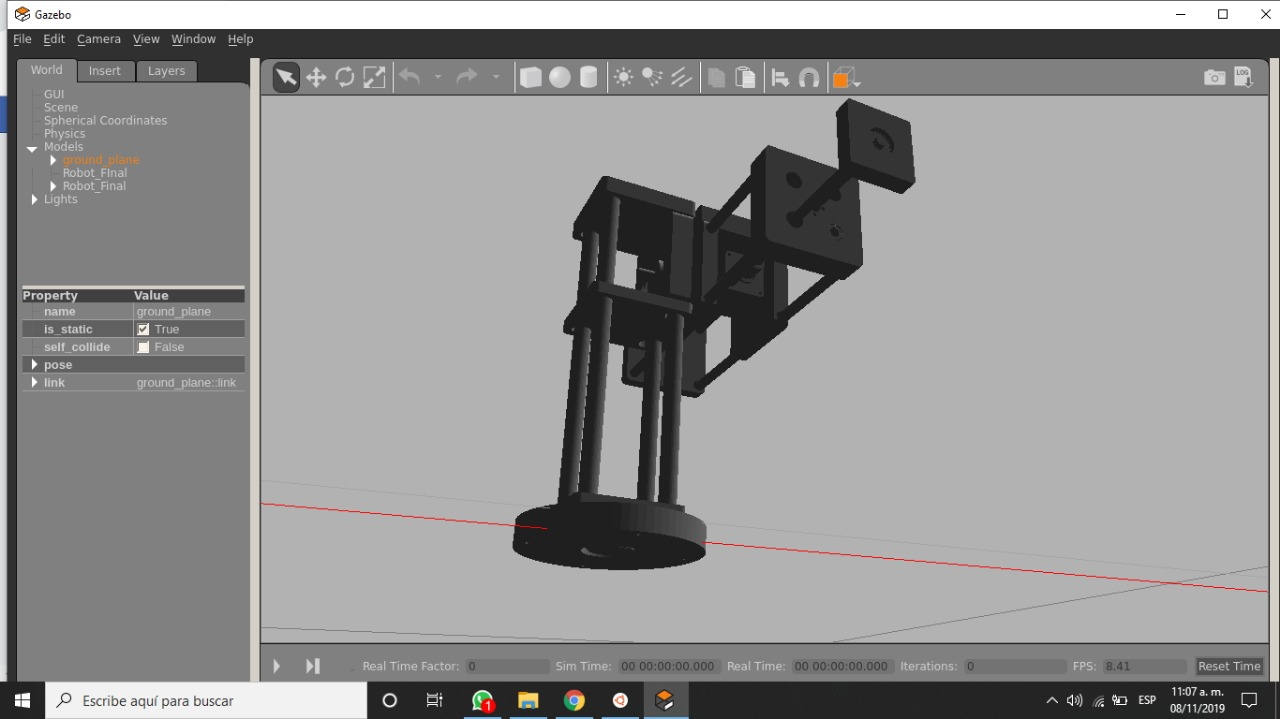
\includegraphics[scale=.30]{101.png}
\end{center}
\caption{Prototipo del Robot.}
\label{blender}:
\end{figure}


\chapter{Desarrollo}
Primeramente y partiendo del ensamble realizado en SolidWorks, exportamos dicho ensamble como .STL con lo cual el archivo podrá importarse en Blender de manera sencilla por medio de mallas.

\begin{figure}[h]
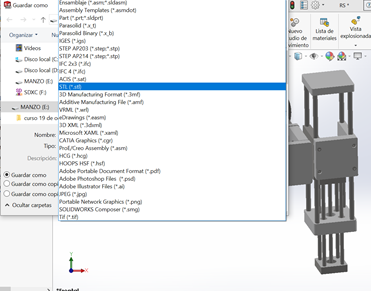
\includegraphics[scale=.9]{1.png}
\caption{Exportación en SolidWorks}
\label{Imagen 1}
\end{figure}
Iniciamos nuestra máquina virtual, donde trabajaremos con el archivo .STL
\begin{figure}[h]
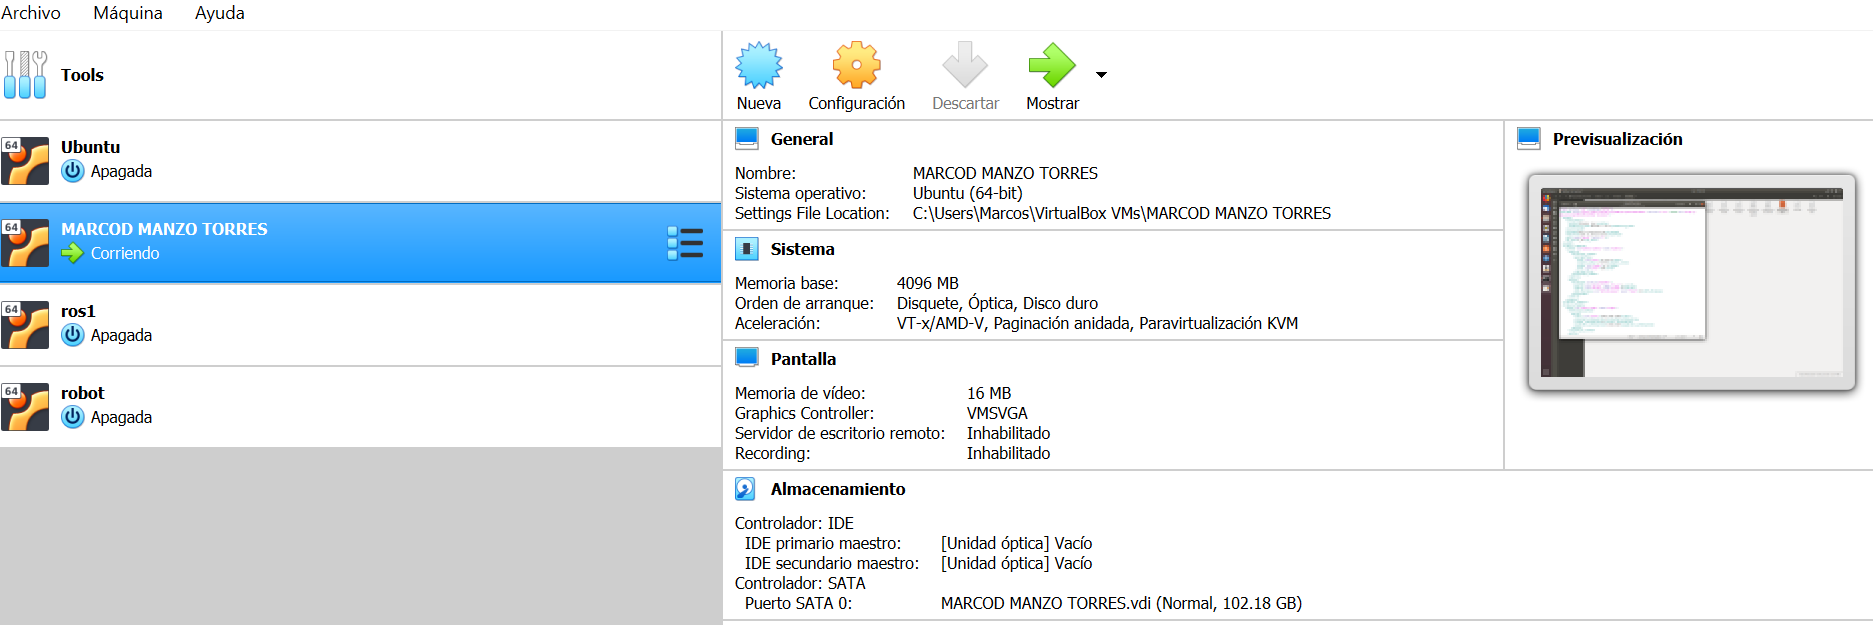
\includegraphics[scale=.7]{maquina.png}
\caption{Inicio de máquina virtual}
\label{Imagen 2}
\end{figure}\\
Abrimos una terminal en nuestro sistema Ubuntu, y colocamos el nombre de blender para abrir el programa y comenzar a trabajar.

\begin{figure}[h]
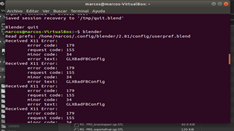
\includegraphics[scale=1.9]{2.png}	\caption{Inicio de Blender}
\label{Imagen 3}
\end{figure}
Tras haber exportado el archivo .STL de SolidWorks, lo importamos en Blender y observamos que el ensamble está subdividido por cada unas de las piezas que lo conforman
\begin{figure}[h]
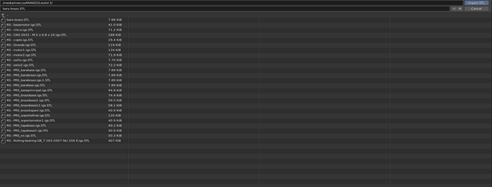
\includegraphics[scale=1.7]{3.png}
\caption{Archivos .STL}
\label{Imagen 4}
\end{figure}\\
Una vez abrimos el ensamble, observamos que nos faltan algunas piezas las cuales se colocan de manera manual por medio de la opción transformar y por medio de coordenadas, se colocan en el lugar deseado.
\begin{figure}[h]
	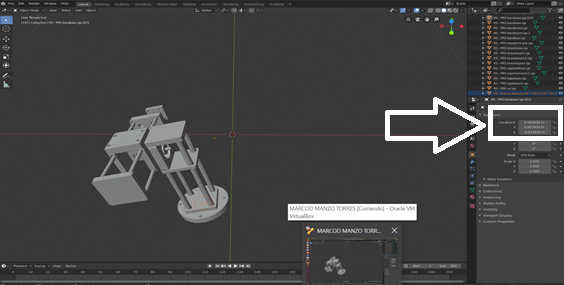
\includegraphics[scale=1.2]{4.png}
	\caption{Ensamble importado}
	\label{Imagen 4}
\end{figure}\\
Ahora que finalizamos el ensamble importado en Blender, guardamos el mismo como archivo .DAE y lo colocamos en nuestra carpeta launcher de Gazebo
\begin{figure}[h]
	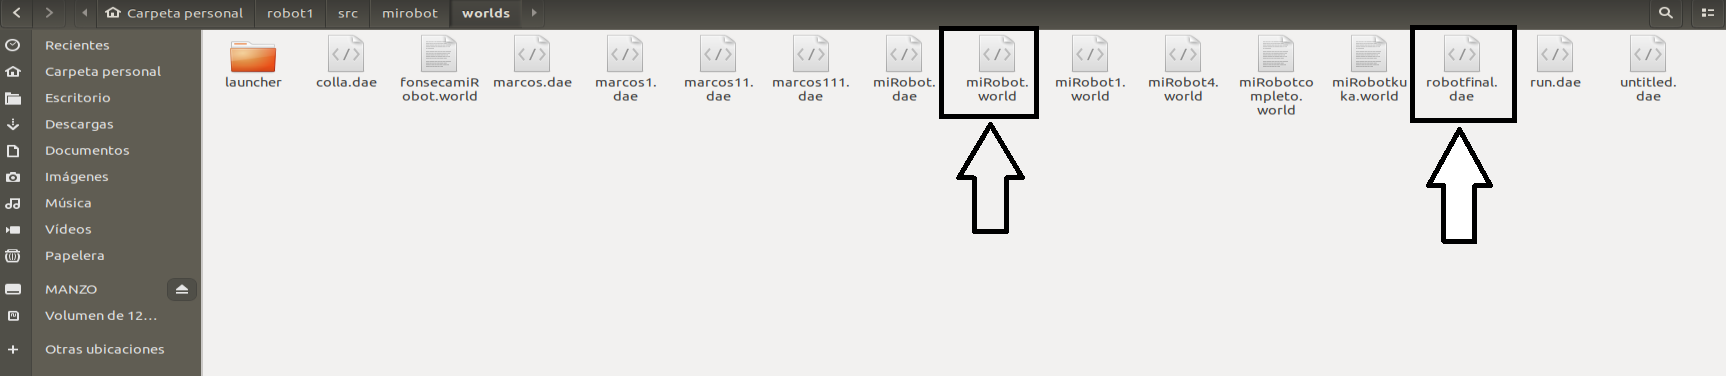
\includegraphics[scale=.5]{carpeta.png}
	\caption{Guardar ensamble}
	\label{Imagen 5}
\end{figure}\\
Observamos la información almacenada en nuestro archivo .DAE, donde nuestro ensamble fue guardado por medio de mallas similar a un archivo .USDF que es el archivo base de Gazebo.
Encontramos cómo se declara el entorno y las uniones para que estas aparescan a la hora de correr el mismo.
\begin{figure}[h]
	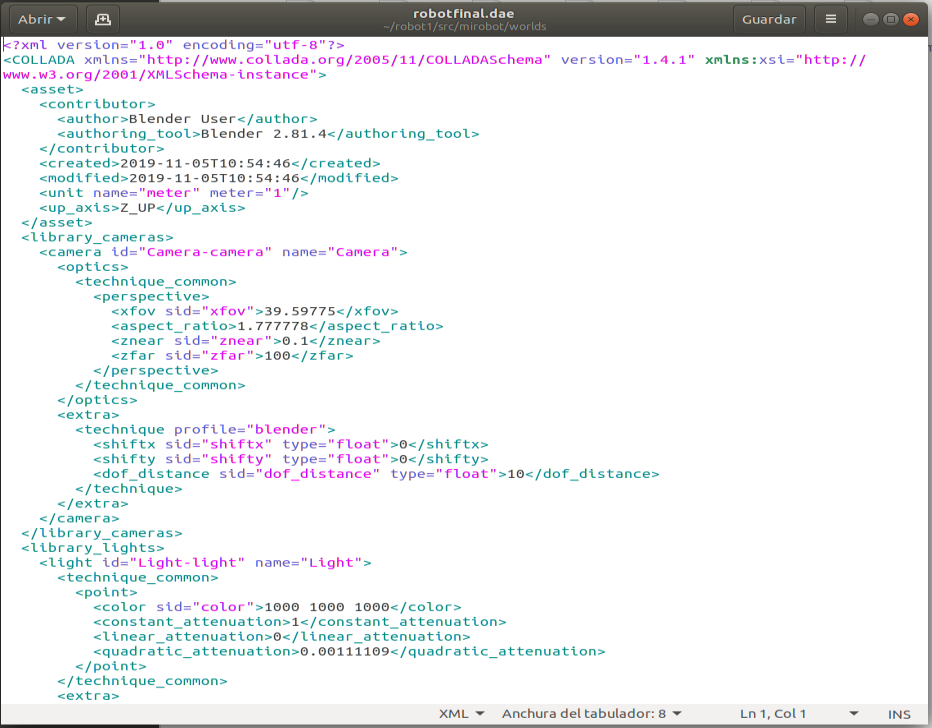
\includegraphics[scale=.45]{dae.png}
	\caption{Archivo .DAE}
	\label{Imagen 6}
\end{figure}\\
Para iniciar el contenido en Gazebo, necesitamos declarar un archivo .World el cual funciona como launcher para iniciar el contenido o arrancar el contenido especificado. solo basta con colocar el nombre del archivo .DAE que deseamos iniciar.
\begin{figure}[h]
	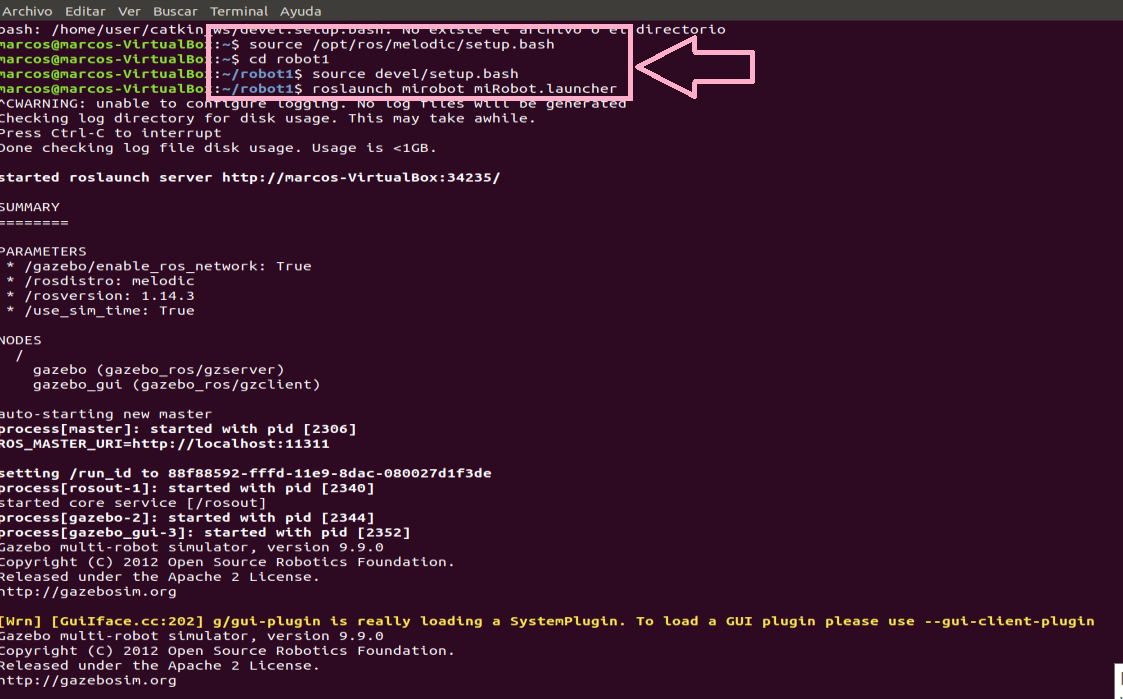
\includegraphics[scale=.45]{6.png}
	\caption{Arrancador}
	\label{Imagen 7}
\end{figure}
Ahora solo basta abrir un terminal, donde iniciaremos gazebo y nos abrirá nuestro archivo colocado en el arrancador y en nuestra carpeta de trabajo.
\begin{figure}[h]
	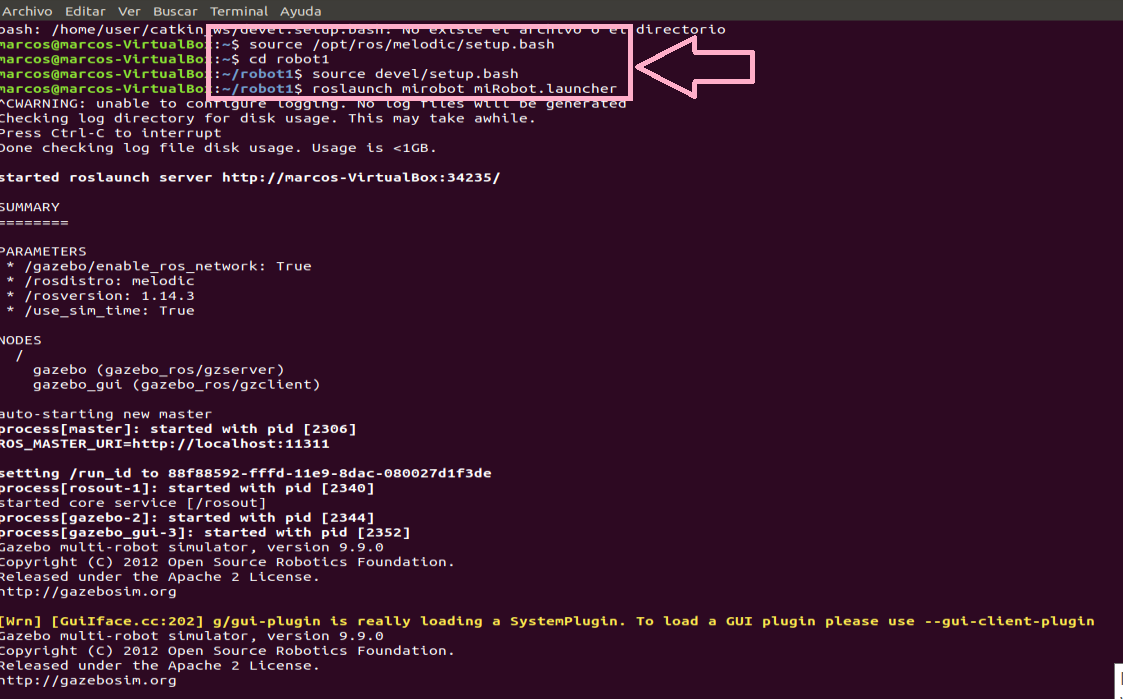
\includegraphics[scale=.75]{iniciargaz.png}
	\caption{Iniciar Gazebo}
	\label{Imagen 8}
\end{figure}\\
Tras haber iniciado Gazebo en nuestra terminal, podemos observar una ventana nueva donde nos aparece el contenido y su entorno, además de poder observar a detalle la simluación de nuestro robot.
\begin{figure}[h]
	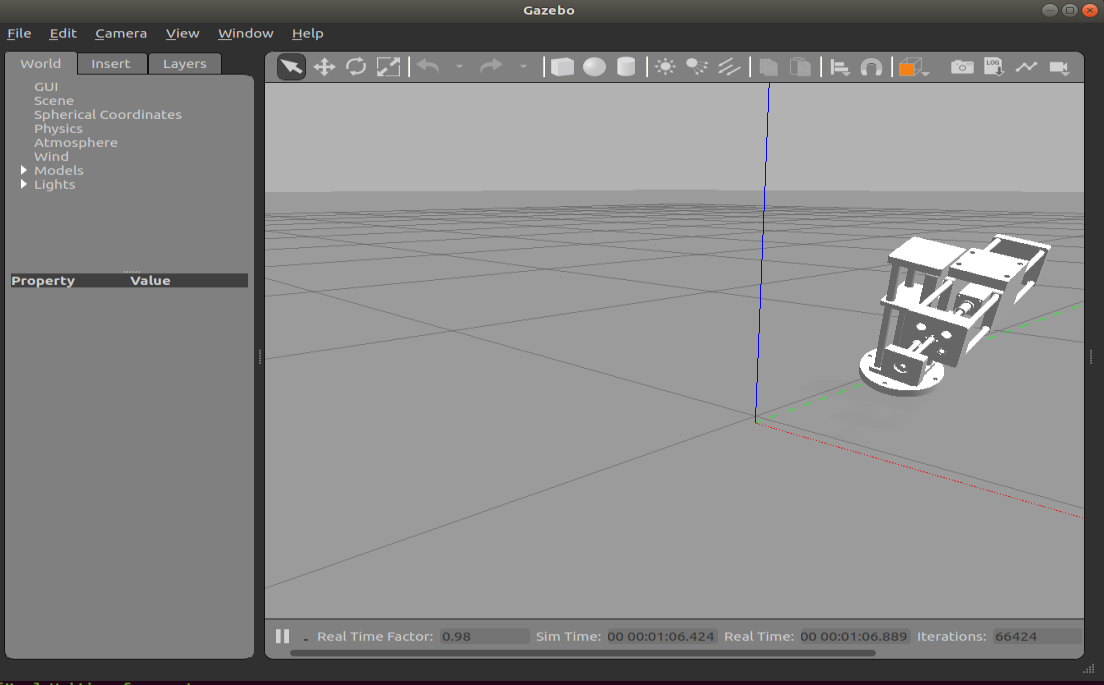
\includegraphics[scale=.75]{gaz.png}
	\caption{Gazebo}
	\label{Imagen 9}
\end{figure}
\chapter{Simulado}
Simulador 3D Gazebo
Gazebo es un simulador de entornos 3D que posibilita evaluar el comportamiento de un robot en un mundo virtual. Permite, entre muchas otras opciones, diseñar robots de forma personalizada, crear mundos virtuales usando sencillas herramientas CAD e importar modelos ya creados.

Además, es posible sincronizarlo con ROS de forma que los robots emulados publiquen la información de sus sensores en nodos, así como implementar una lógica y un control que dé ordenes al robot.\\
Gazebo forma parte del bundle de ros "ros-kinetic-desktop-full", no obstante el robot que se usará como ejemplo no está integrado. El robot al que nos referimos es Turtlebot, un pequeño robot con una estructura montada sobre una base de Roomba y que integra sensores de odometría y una cámara RGB-D, entre otros.
\begin{figure}
\begin{center}
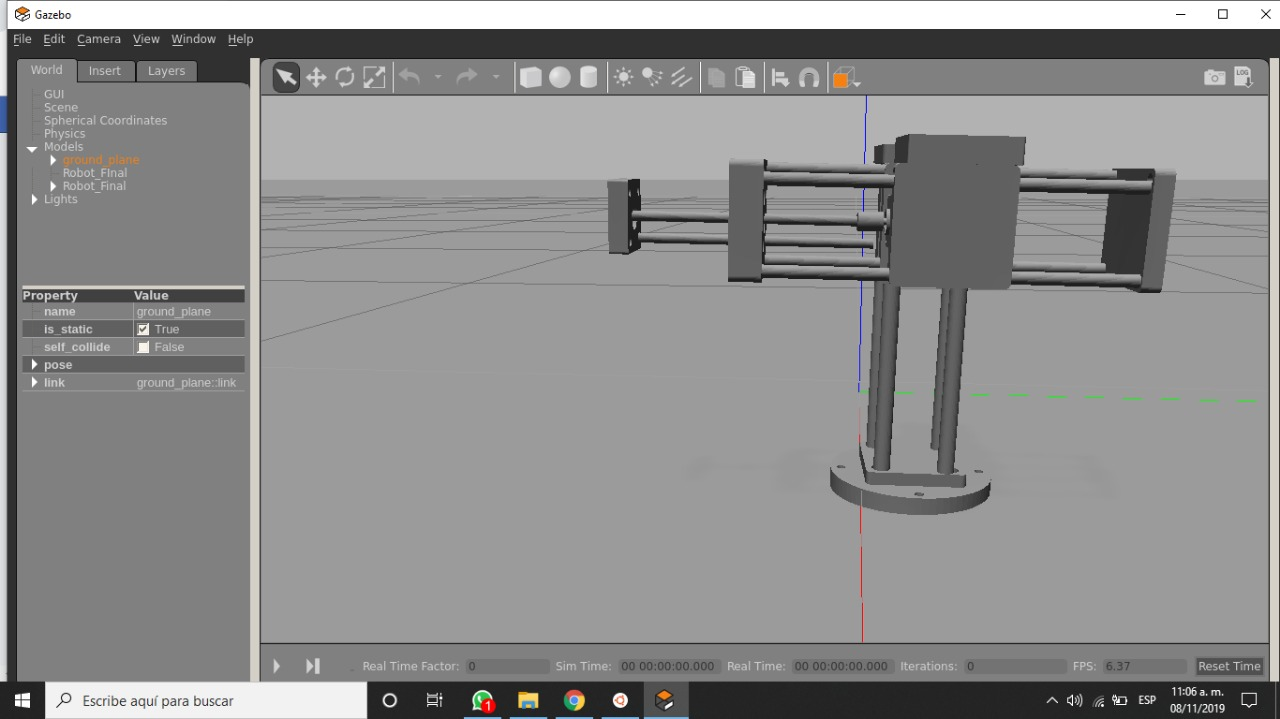
\includegraphics[scale=.30]{102.jpeg}
\end{center}
\caption{Orentación.}
\label{blender}:
\end{figure}
El proceso de instalación se detalla en la Wiki de ROS, donde además se encuentra toda la documentación y otros tutoriales de interés.
\chapter{Control de la cámara}
El control del punto de vista de diseño es parecido al que muestran otros programas de diseño o simulación 3D:\\

  El botón izquierdo del ratón sirve para trasladar la cámara por el mundo.\\
  El botón derecho o la rueda del ratón sirve para hacer zoom en la escena\\
  El botón central del ratón sirve para rotar la cámara\\
  
Diseño de mundos\\
Gazebo permite diseñar elementos con herramientas CAD, dichas herramientas son muy limitadas, pero suficientes para crear mundos sencillos.
Estas herramientas están situadas en la zona superior del programa y nos permite insertar cubos, esferas y cilindros, así como distintos puntos de luz.\\
Los elementos que contiene el mundo se van listando en la parte izquierda del programa, bajo la pestaña "World" y si son seleccionados permiten la edición de algunas propiedades tales como la pose o el nombre (esta característica no está implementada en la versión de que disponemos en el laboratorio).\\
\chapter{Mover el Robot por el mundo virtual usando comandos de velocidad}
La forma de mover los robots, tanto en el mundo real como en el simulador, es enviándoles comandos de velocidad. Los robots tienen un nodo que consumen mensajes de tipo geometry msgs Twist que son el tipo de mensajes para indicar precisamente eso, valores para velocidades lineales y angulares.\\

\begin{figure}
\begin{center}
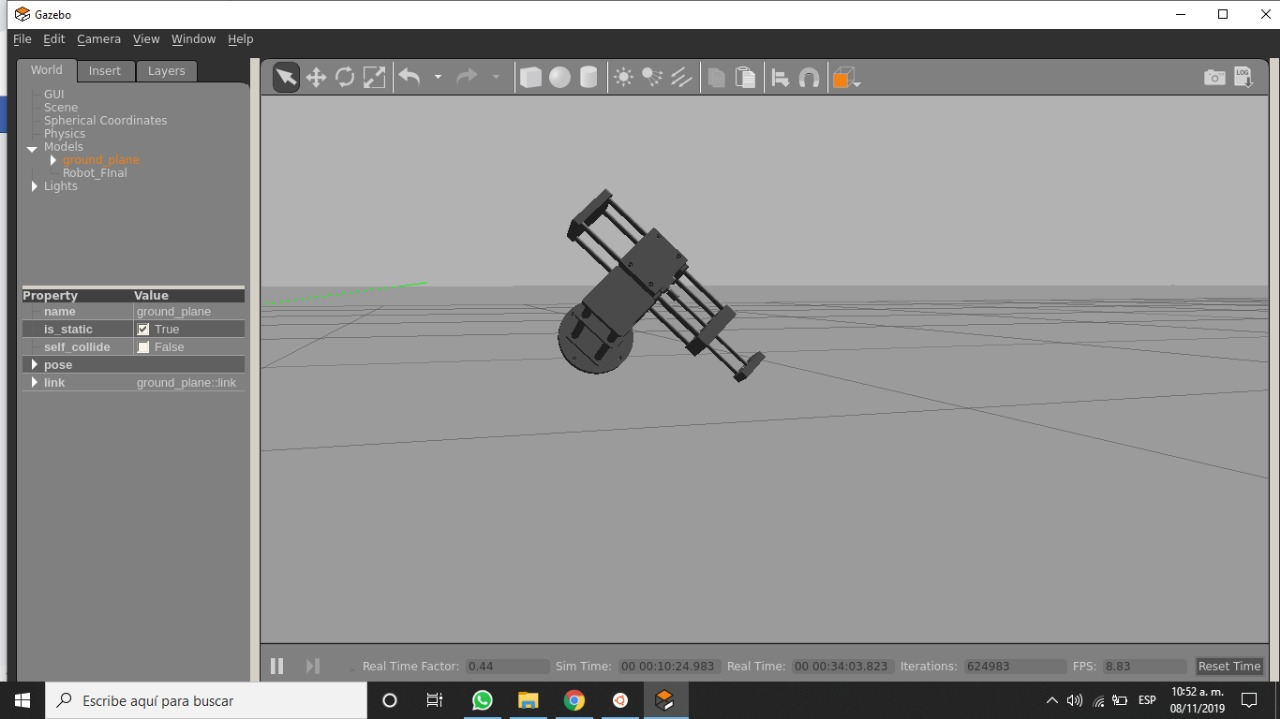
\includegraphics[scale=.30]{106.jpeg}
\end{center}
\caption{Primeros Movimientos.}
\label{blender}:
\end{figure}
En este bloque vamos a aprender cómo mover el Robot mandándole comandos de velocidad tal y como hacíamos en la sección Mover a turtlebot por el mundo virtual usando comandos de velocidad pero en este caso en vez de mandarle el mensaje directamente desde la terminal lo haremos desde un nodo ROS. Las ventajas de este sistema son evidentes: podremos reunir la información de los sensores para averiguar la situación del robot y el estado del entorno, procesar estos datos y generar los comandos de movimiento necesarios para guiar el robot en función de la sensorización.\\


Un mensaje de este tipo acepta como máximo 6 valores: las velocidades lineales en x, y, z y las velocidades angulares de roll, pitch y yaw. Estos valores permiten dar movimiento a robots con hasta 6 grados de libertad, pero turtlebot sólo puede moverse por el plano XY y rotar en el eje Z (yaw).
Pero antes de enviar nada es necesario averiguar qué tópico es que acepta este tipo de mensajes por lo que usamos el siguiente comando para ver qué tópicos tenemos en el sistema.

\begin{figure}
\begin{center}
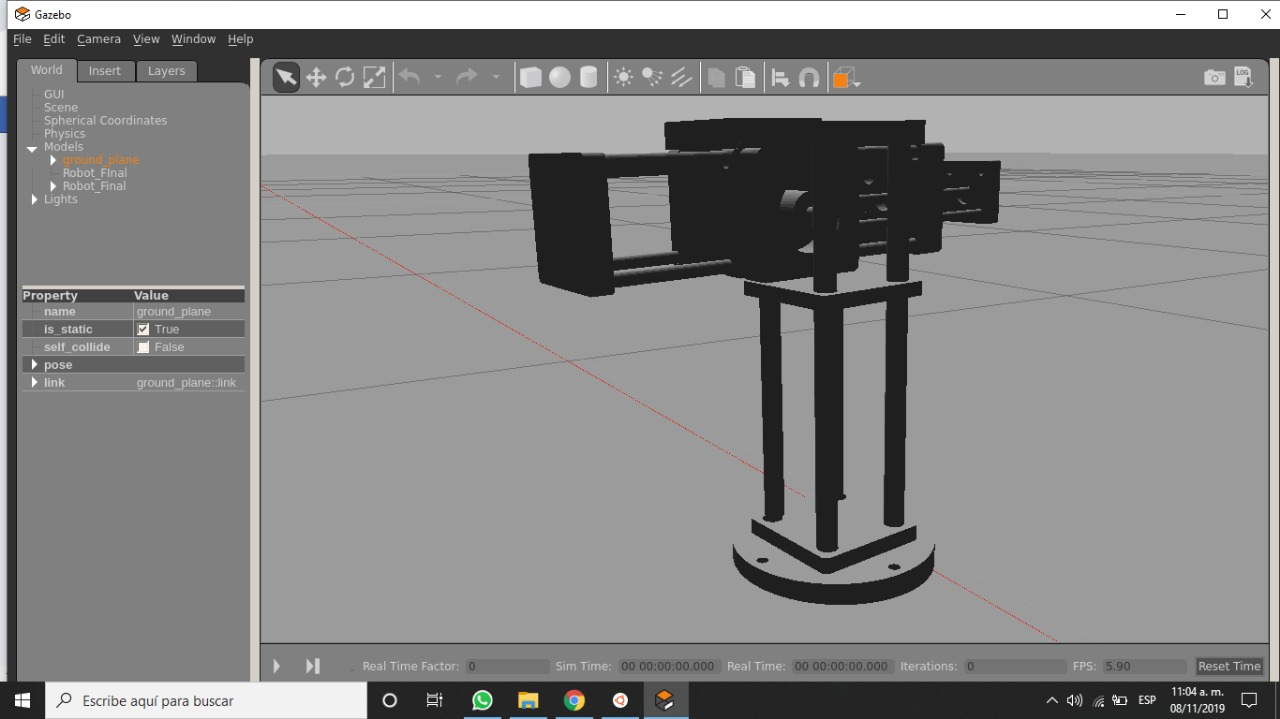
\includegraphics[scale=.30]{103.jpeg}
\end{center}
\caption{Direccionando Movimientos.}
\label{blender}:
\end{figure}

\begin{figure}
\begin{center}
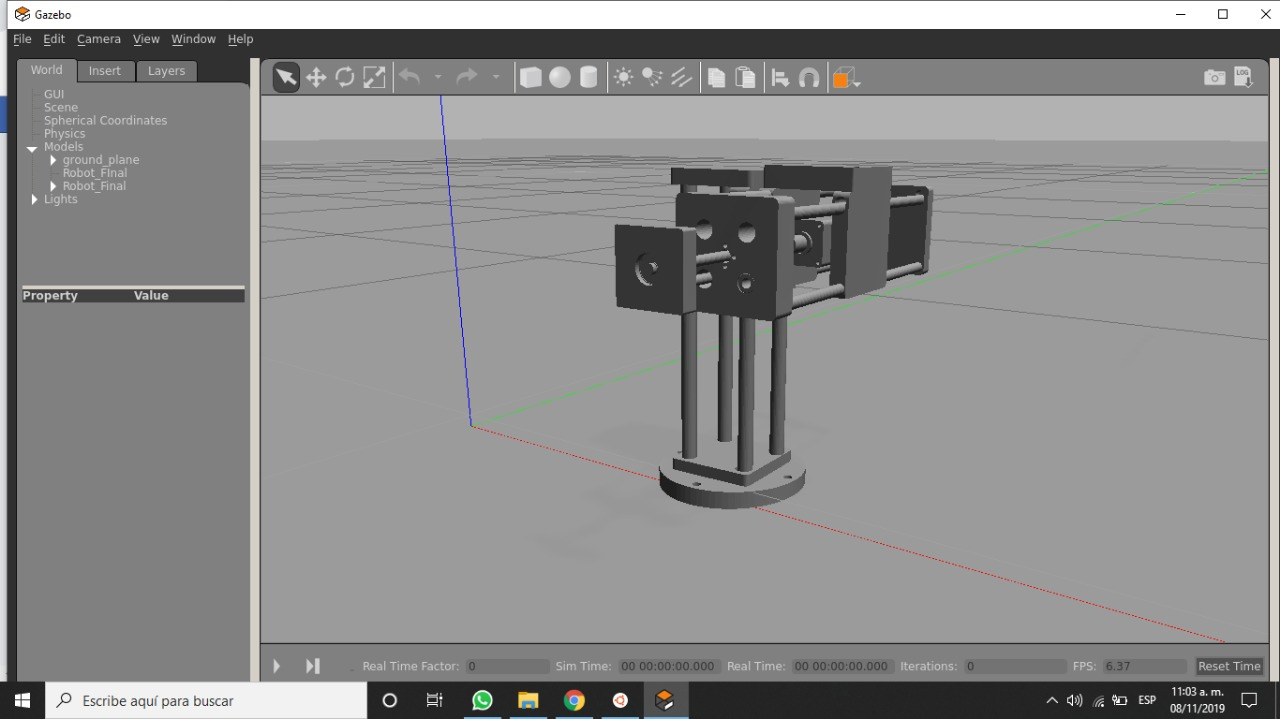
\includegraphics[scale=.30]{105.jpeg}
\end{center}
\caption{Acomodando Dirección.}
\label{blender}:
\end{figure}

\begin{figure}
\begin{center}
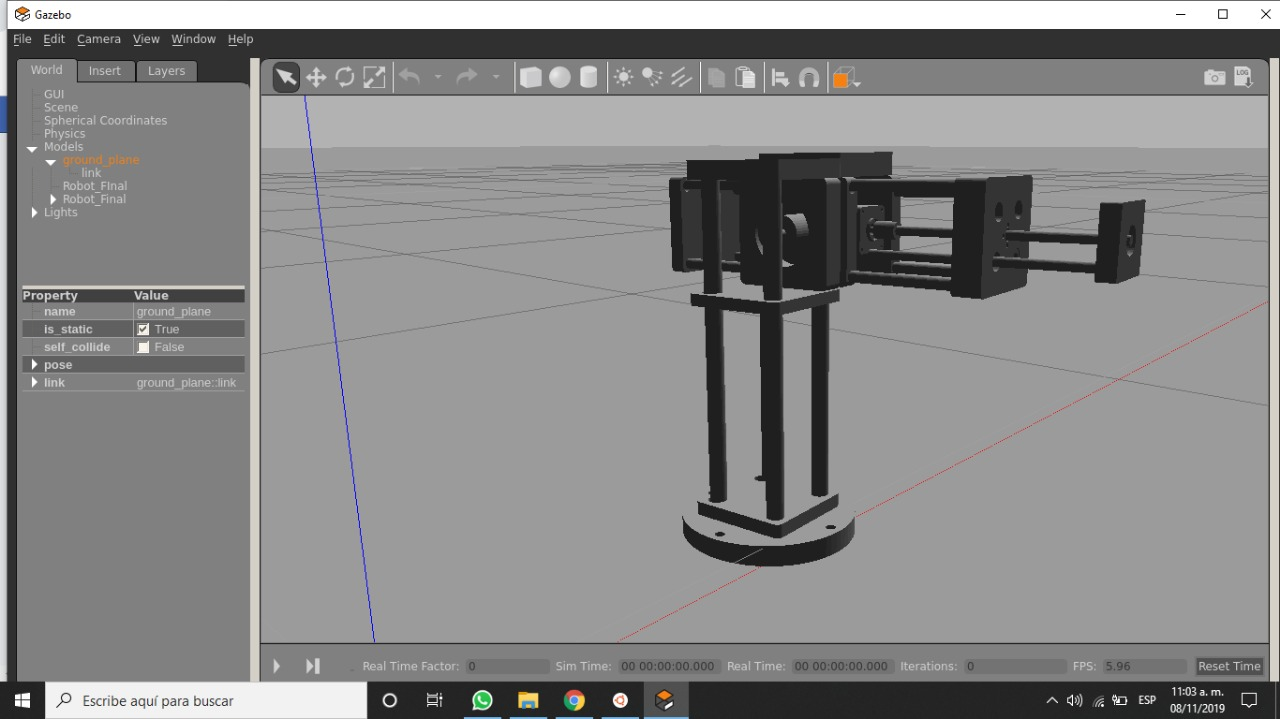
\includegraphics[scale=.30]{104.jpeg}
\end{center}
\caption{Prototipo Moviendose.}
\label{blender}:
\end{figure}

\chapter{conclusión}
En la practica, consistía en familiarizarse con el simulador Gazebo, pues tampoco
se conocía su funcionamiento completamente. De igual manera
que con ROS, tras la labor de investigación llevada a cabo y el trabajo desarrollado, se
considera superado este objetivo. Siendo capaces de simular un entorno y un robot en
él correctamente, y comprendiendo el funcionamiento del programa.
Por último, logramos ser capaces de integrar todas estas herramientas para que
interactuasen entre ellas. Como ha quedado demostrado, este objetivo también se ha
logrado, siendo capaces de mover el robot en la simulación pasando mensajes desde
nodos de ROS y, de igual manera, siendo capaces de transmitir la información de la
simulación a través de los codigos.


\cite{joseph2018kick}
\cite{de2006robotica}
\hfill
\bibliographystyle{unsrt}
\bibliography{torres}


\end{document}

